\documentclass[10pt, letterpaper]{article}
\usepackage{graphicx}
\usepackage[bottom=1.0in]{geometry}
\topmargin=-0.9in
\oddsidemargin -.3in
\evensidemargin -0.3in
\textwidth=7.0in
%\itemsep= -0.5in
%\parsep= -0.04in

\usepackage[cmex10]{amsmath}



\author{Madhusudan Govindraju 39267182 }
\date{}
\begin{document}
\title{EEL5840  Elements of Machine Intelligence - HW 1}
\maketitle

\section{}
 The figure \ref{fig:Q 1} shows the solution for Question 1

\begin{figure}[h!]
	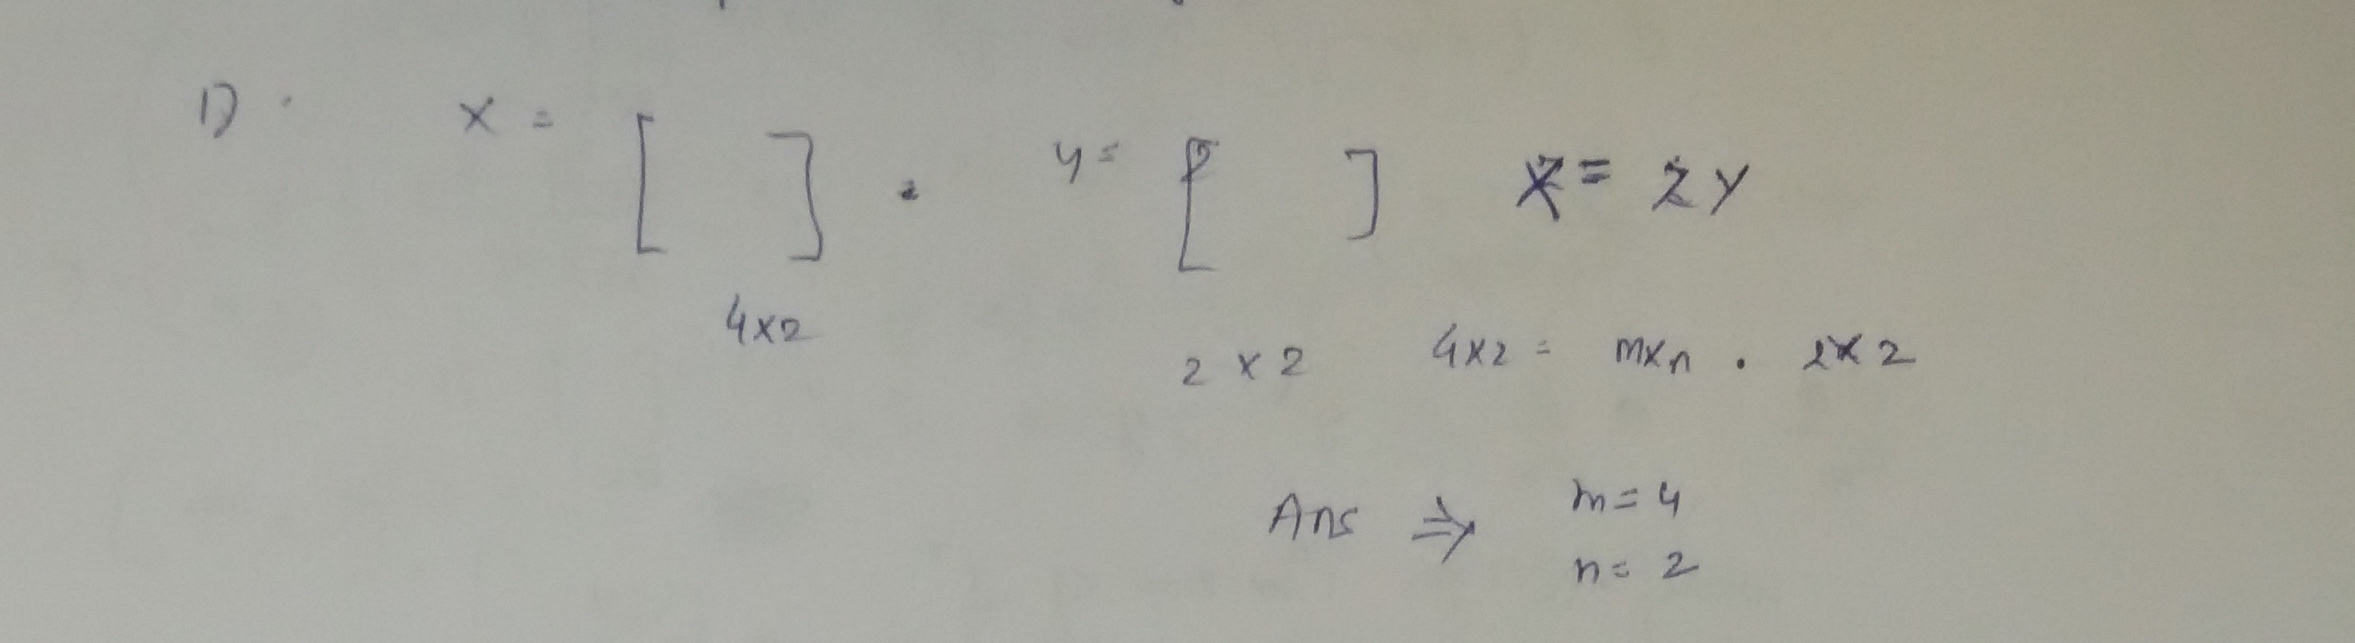
\includegraphics[width=\linewidth]{1.jpg}
	\caption{Q 1}
	\label{fig:Q 1}
\end{figure}


\newpage

\section{}
 The figure \ref{fig:Q 2} shows the solution for Question 2
 \begin{figure}[h!]
	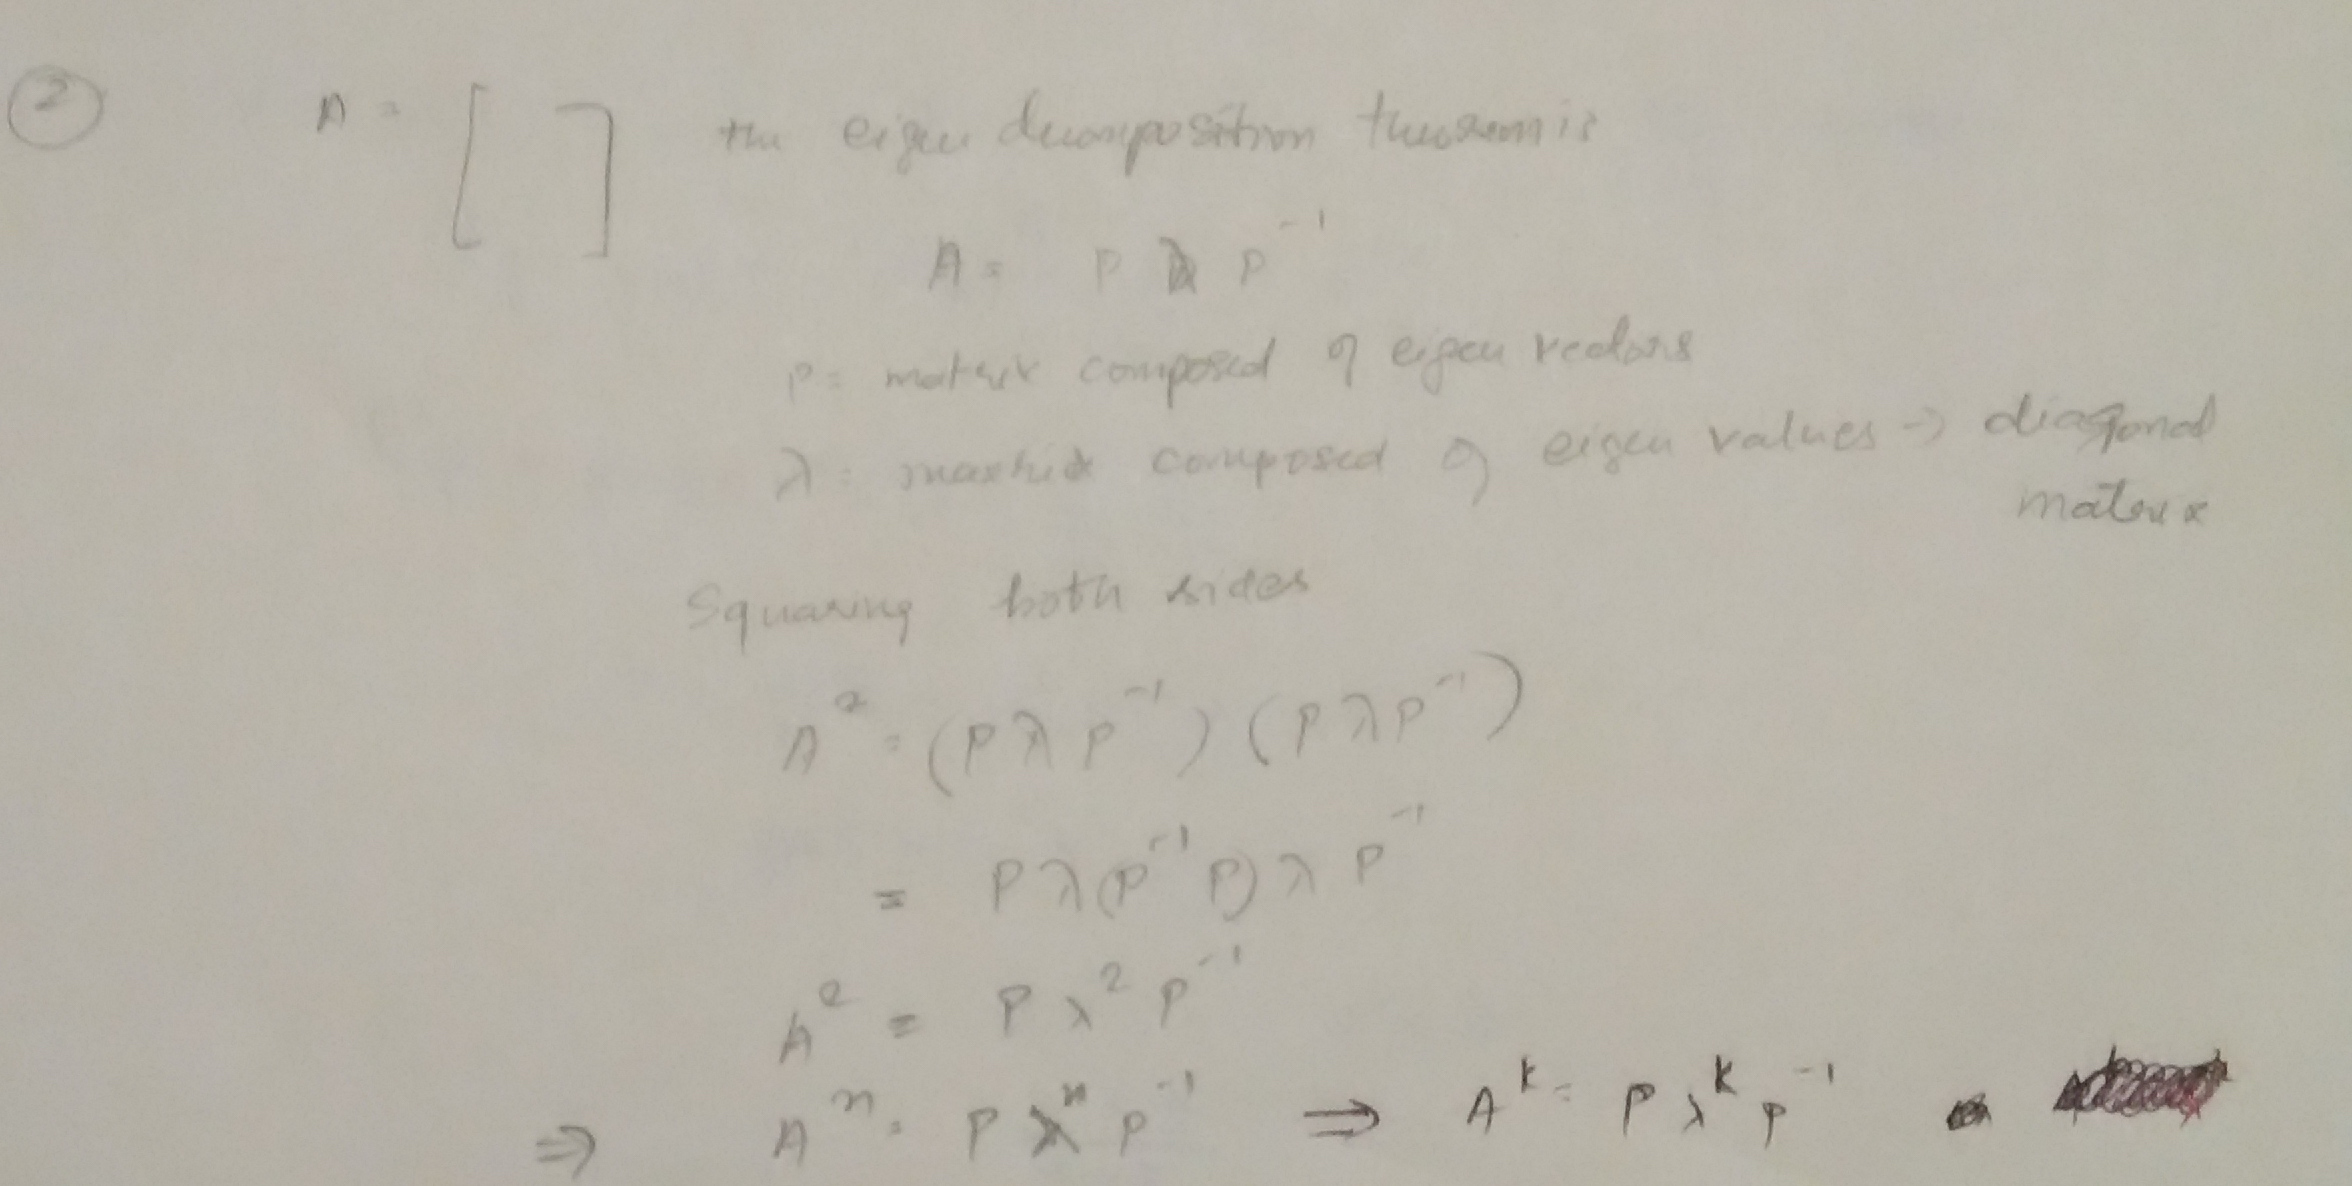
\includegraphics[width=\linewidth]{2.jpg}
	\caption{Q 2}
	\label{fig:Q 2}
\end{figure}
 
 
 %\vspace{100 mm}
 \newpage

\section{} 
The figure \ref{fig:Q 3} shows the solution for Question 3. Using that equation we solve for the given matrices to get the following solution
\begin{verbatim}
>> X = [ -3 1 1 2 0; 2 0 1 4 1; 1 0 0 1 -1];
>> y = [1; -1; 1; 2; 10];
>> w = ((2.* X)* X')^(-1) * ((2.* X)* y)
w =
   -0.9552
    2.7164
   -7.1791
\end{verbatim}

\begin{figure}[h!]
	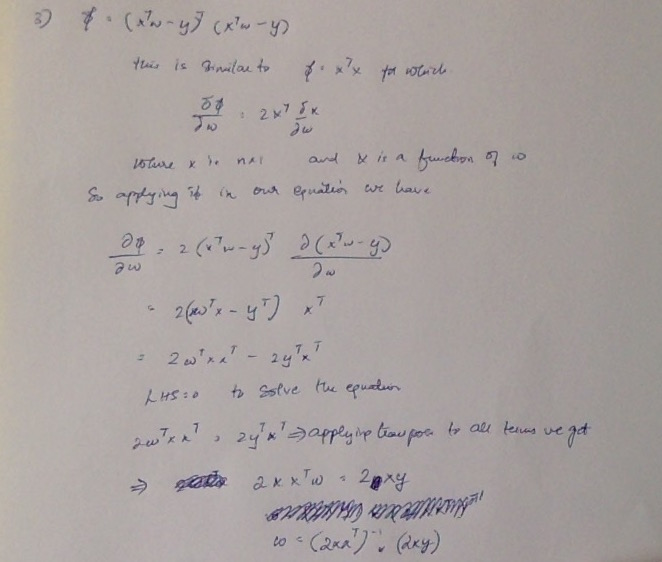
\includegraphics[width=\linewidth]{3.jpg}
	\caption{Q 3}
	\label{fig:Q 3}
\end{figure}

\newpage


\section{}
The figures \ref{fig:Q 4.1} \ref{fig:Q 4.2} \ref{fig:Q 4.3} shows the solution for Question 4.
The principal component can be calculated by 
\begin{verbatim}
>>X = [-1 2 ; 0 0; 2 3]
>>pca(X)

ans =

    -0.7071   0.7071
    0.7071    0.7071
\end{verbatim}

The column corresponding to the largest eigen value is the 1st principal component. In our case the 1st Principal component is the vector [ 0.7071 0.7071]\\ 
From the high error calculated in fig \ref{fig:Q 4.3} we can see that the PCA is not that suitable for this dataset. 
\begin{figure}[h!]
	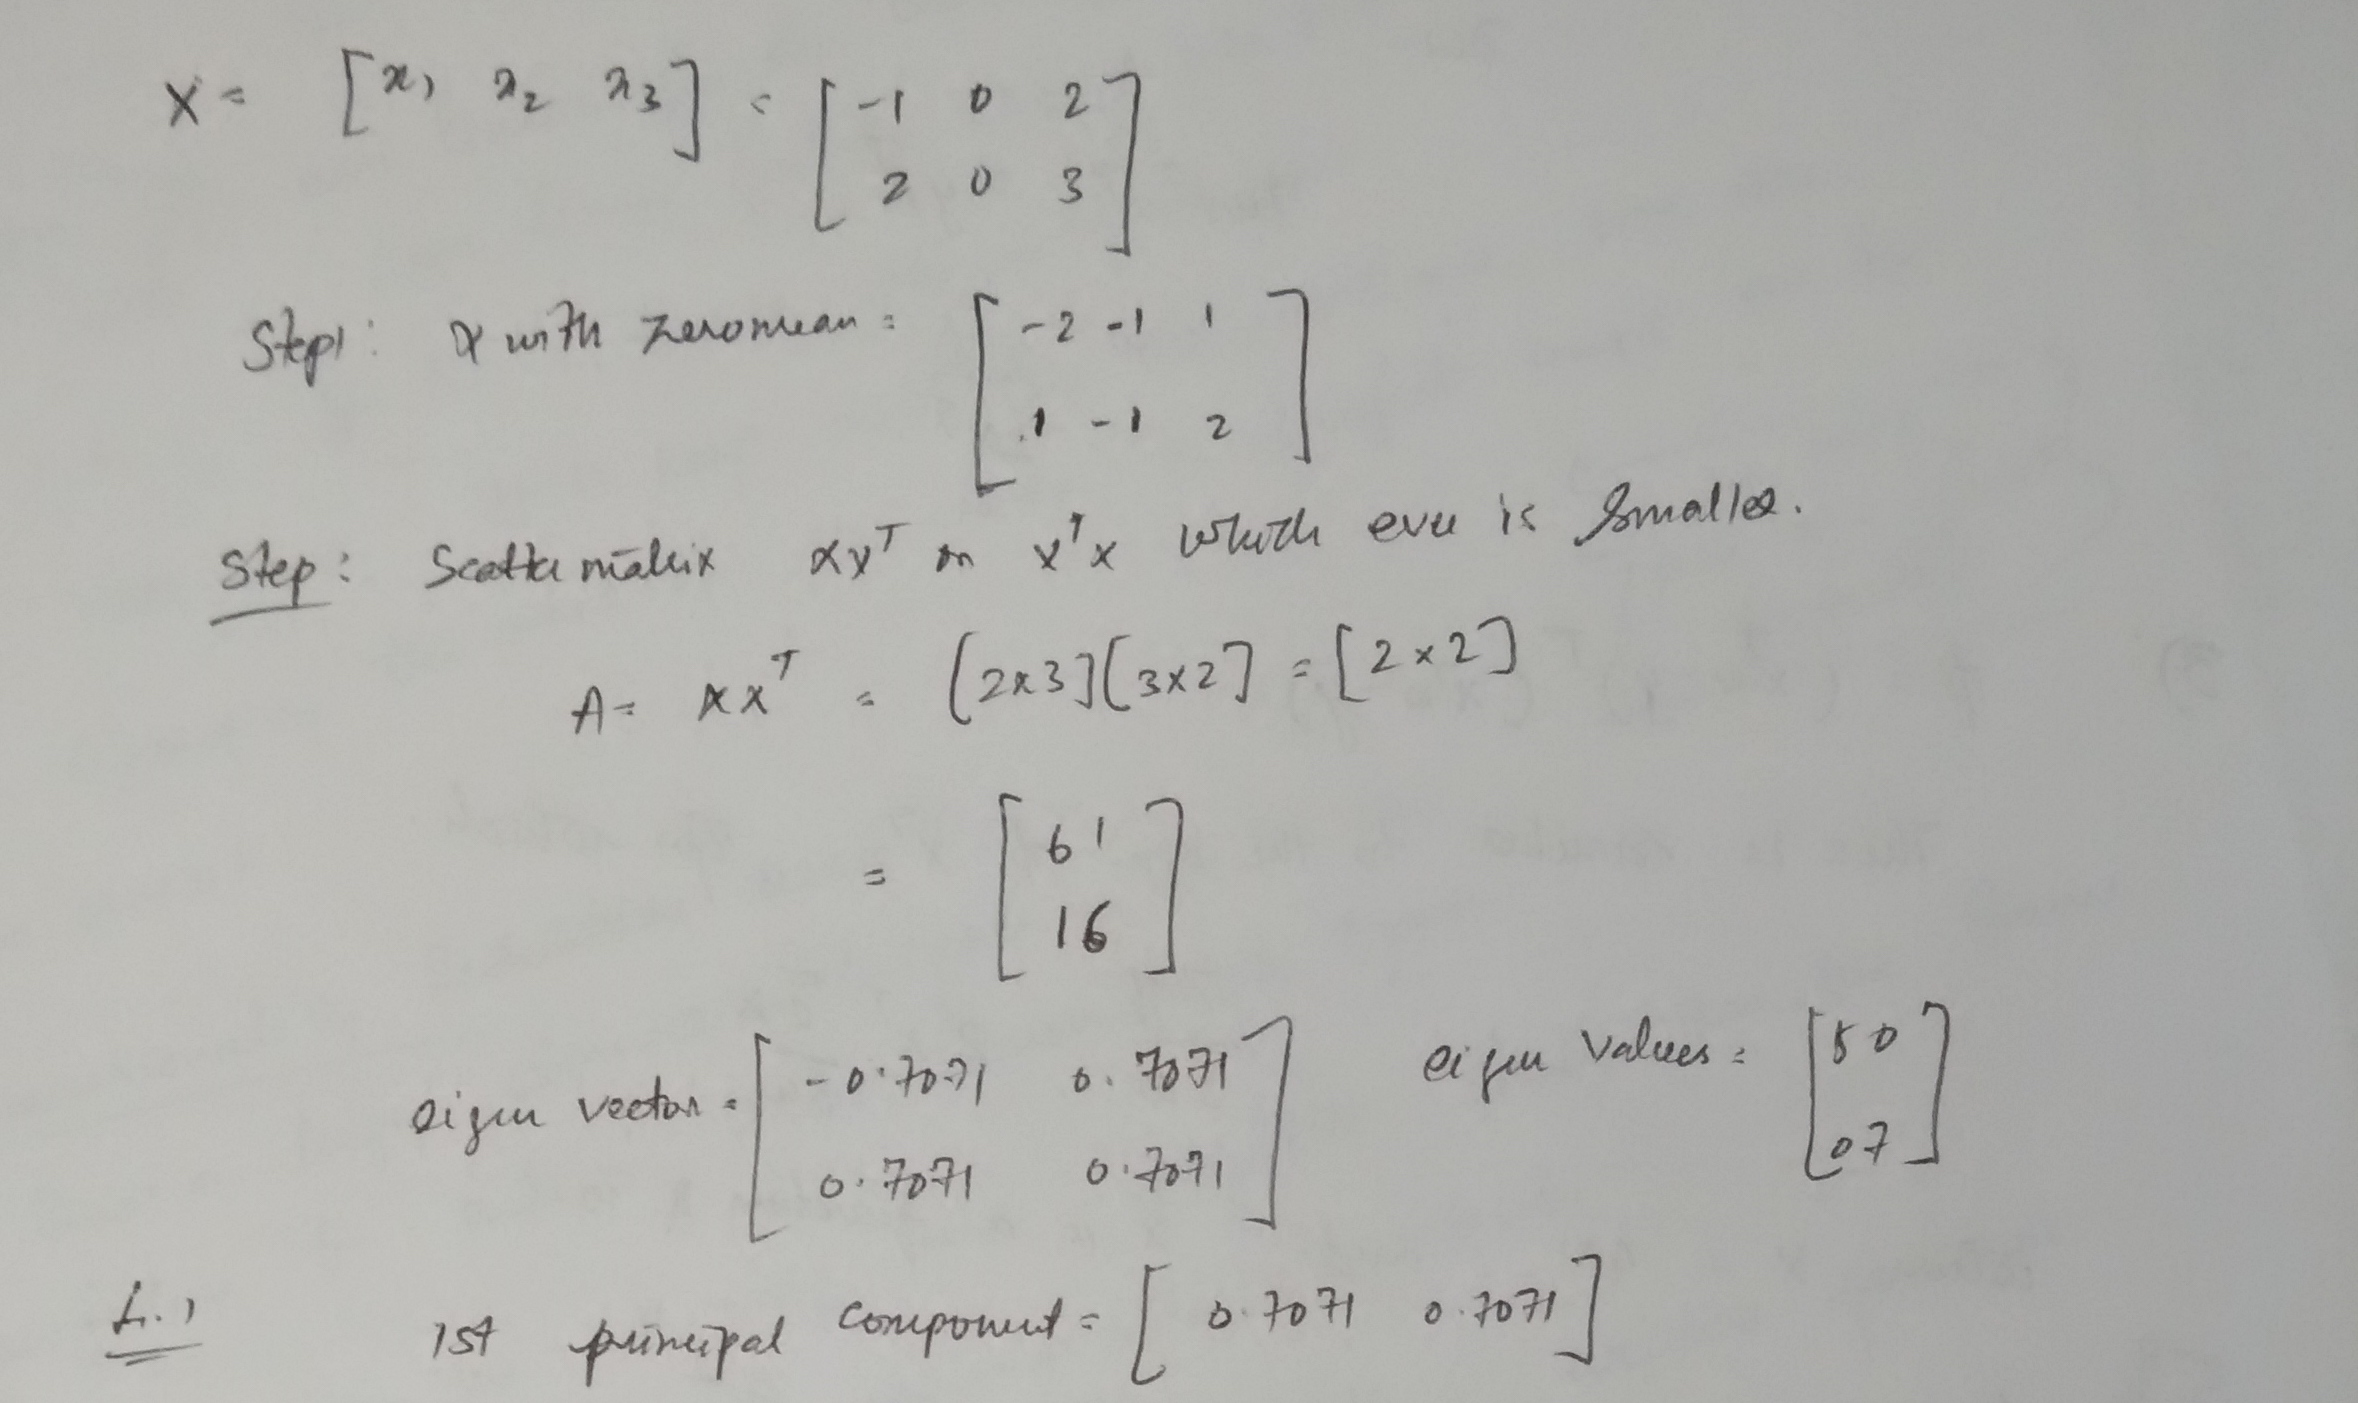
\includegraphics[width=\linewidth]{4_1.jpg}
	\caption{Q 4.1}
	\label{fig:Q 4.1}
\end{figure}
\begin{figure}[h!]
	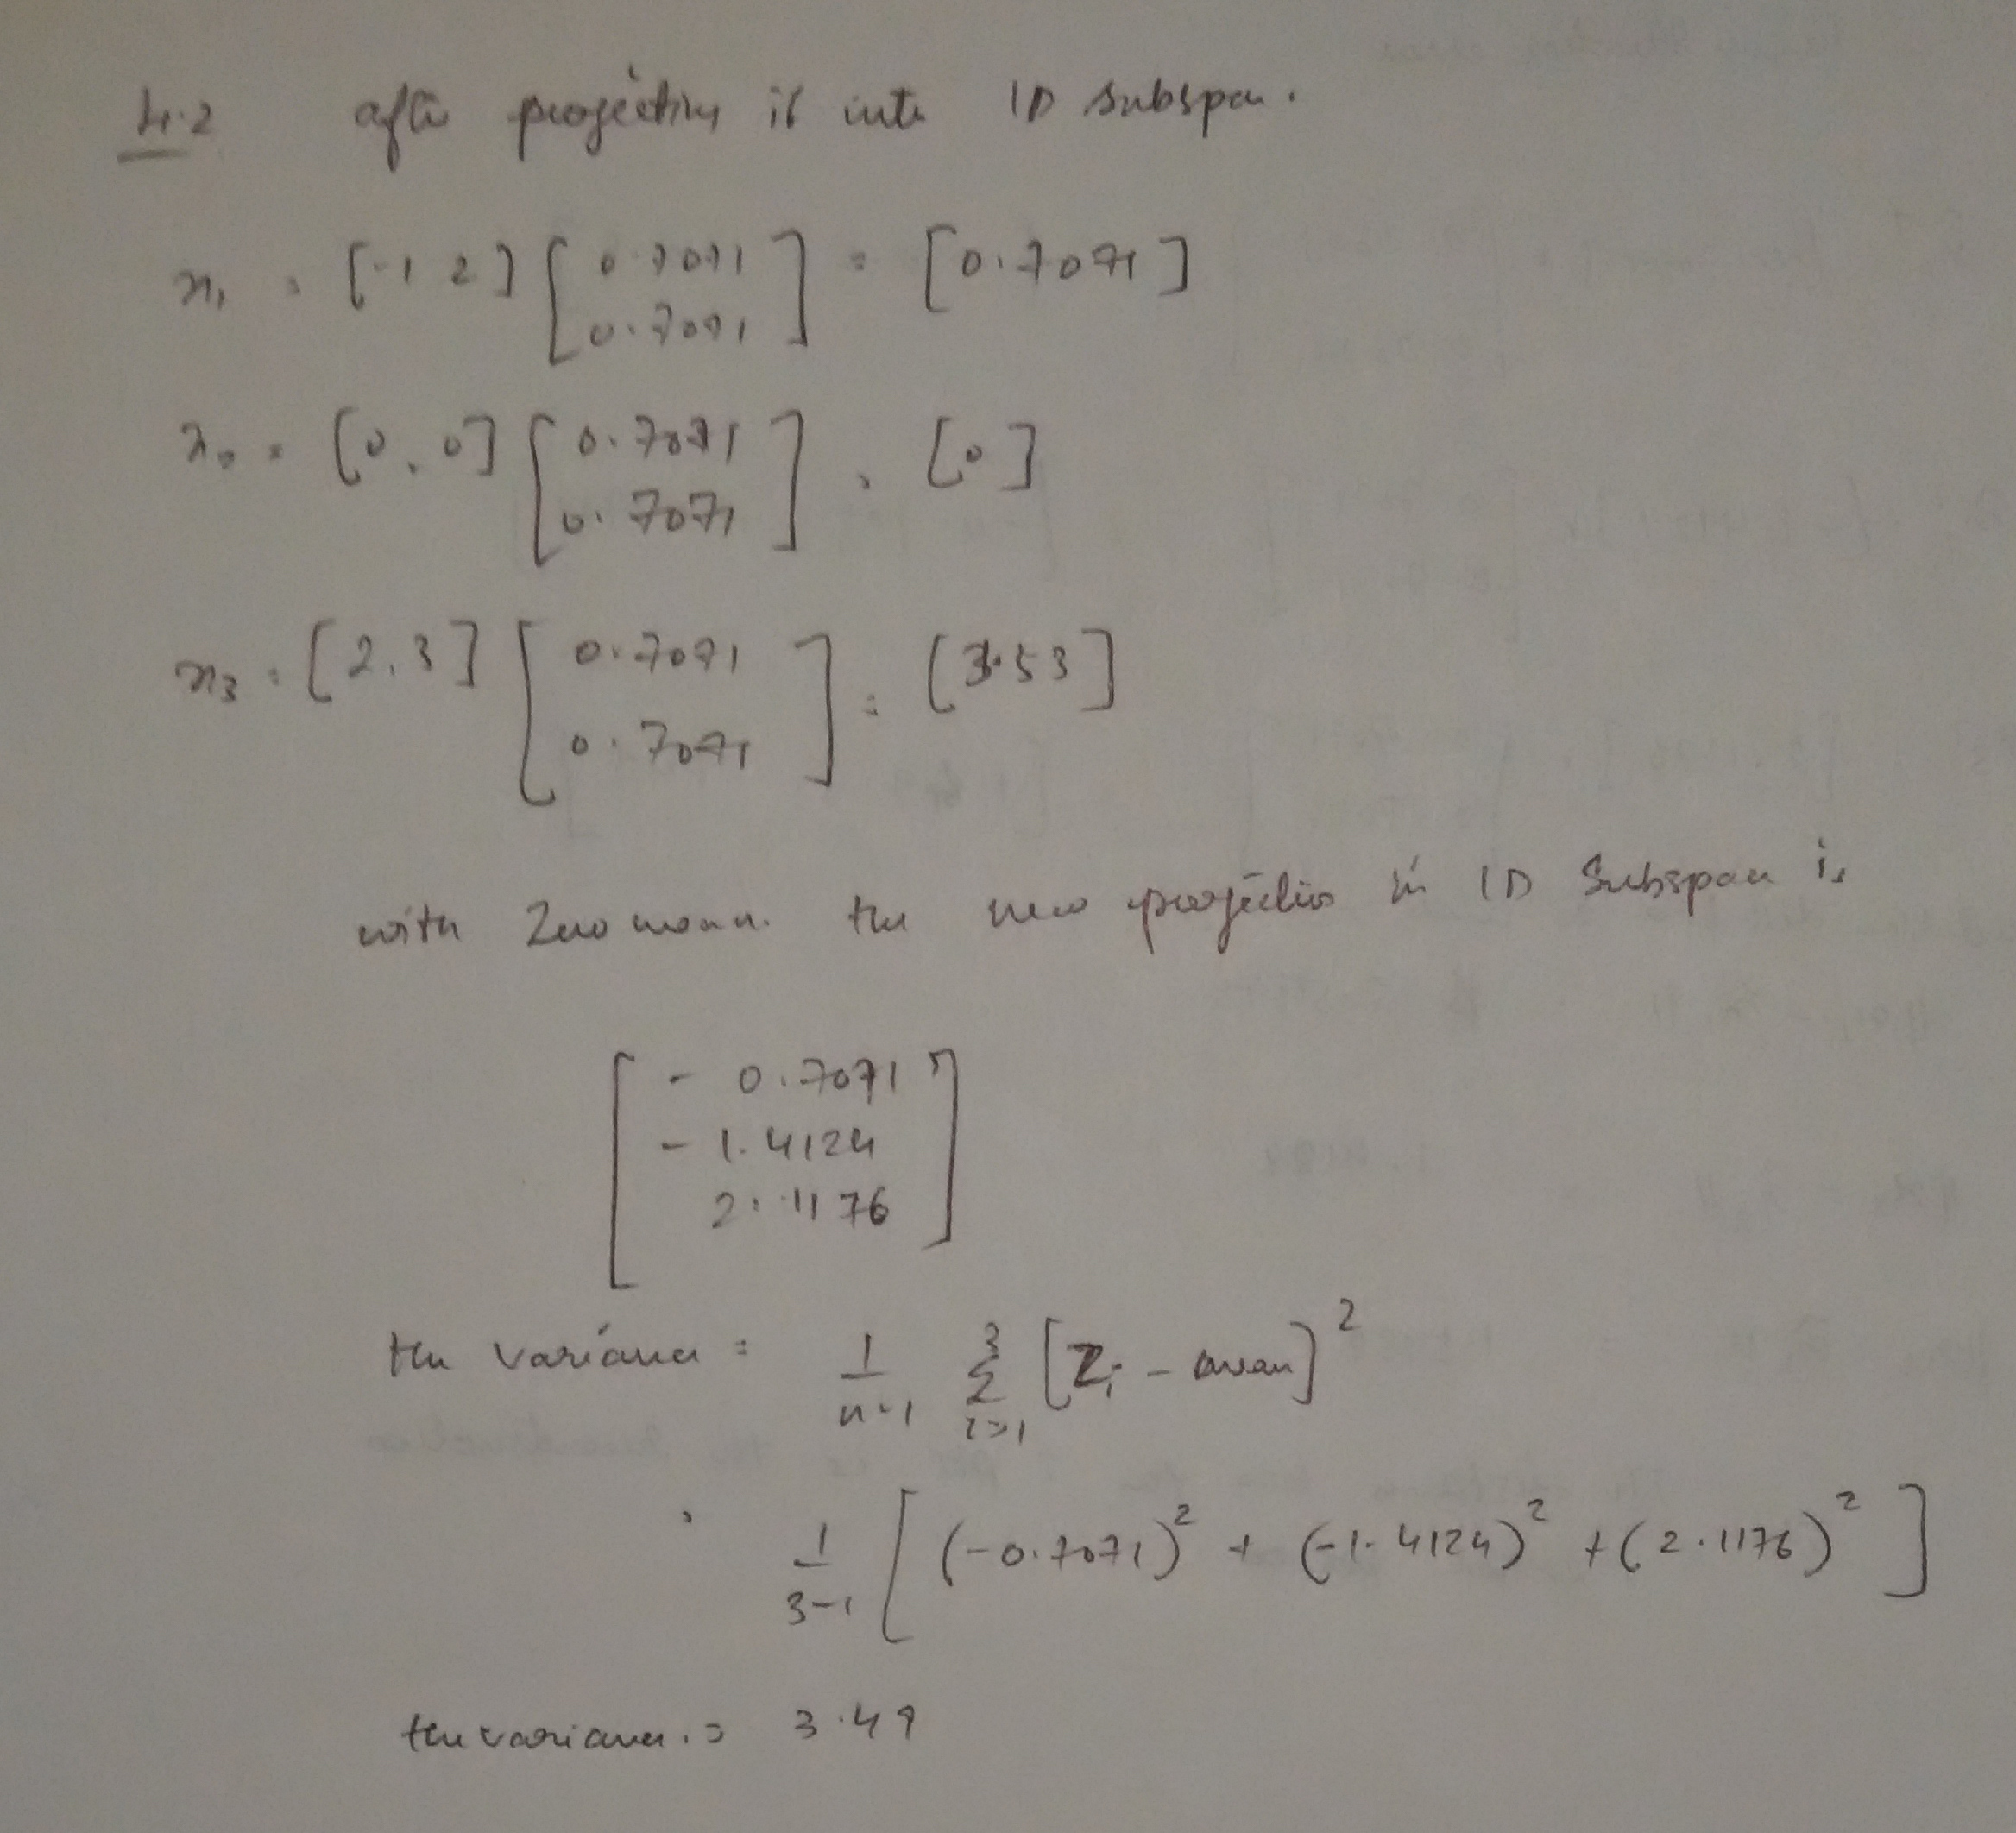
\includegraphics[width=\linewidth]{4_2.jpg}
	\caption{Q 4.2}
	\label{fig:Q 4.2}
\end{figure}


\begin{figure}[h!]
	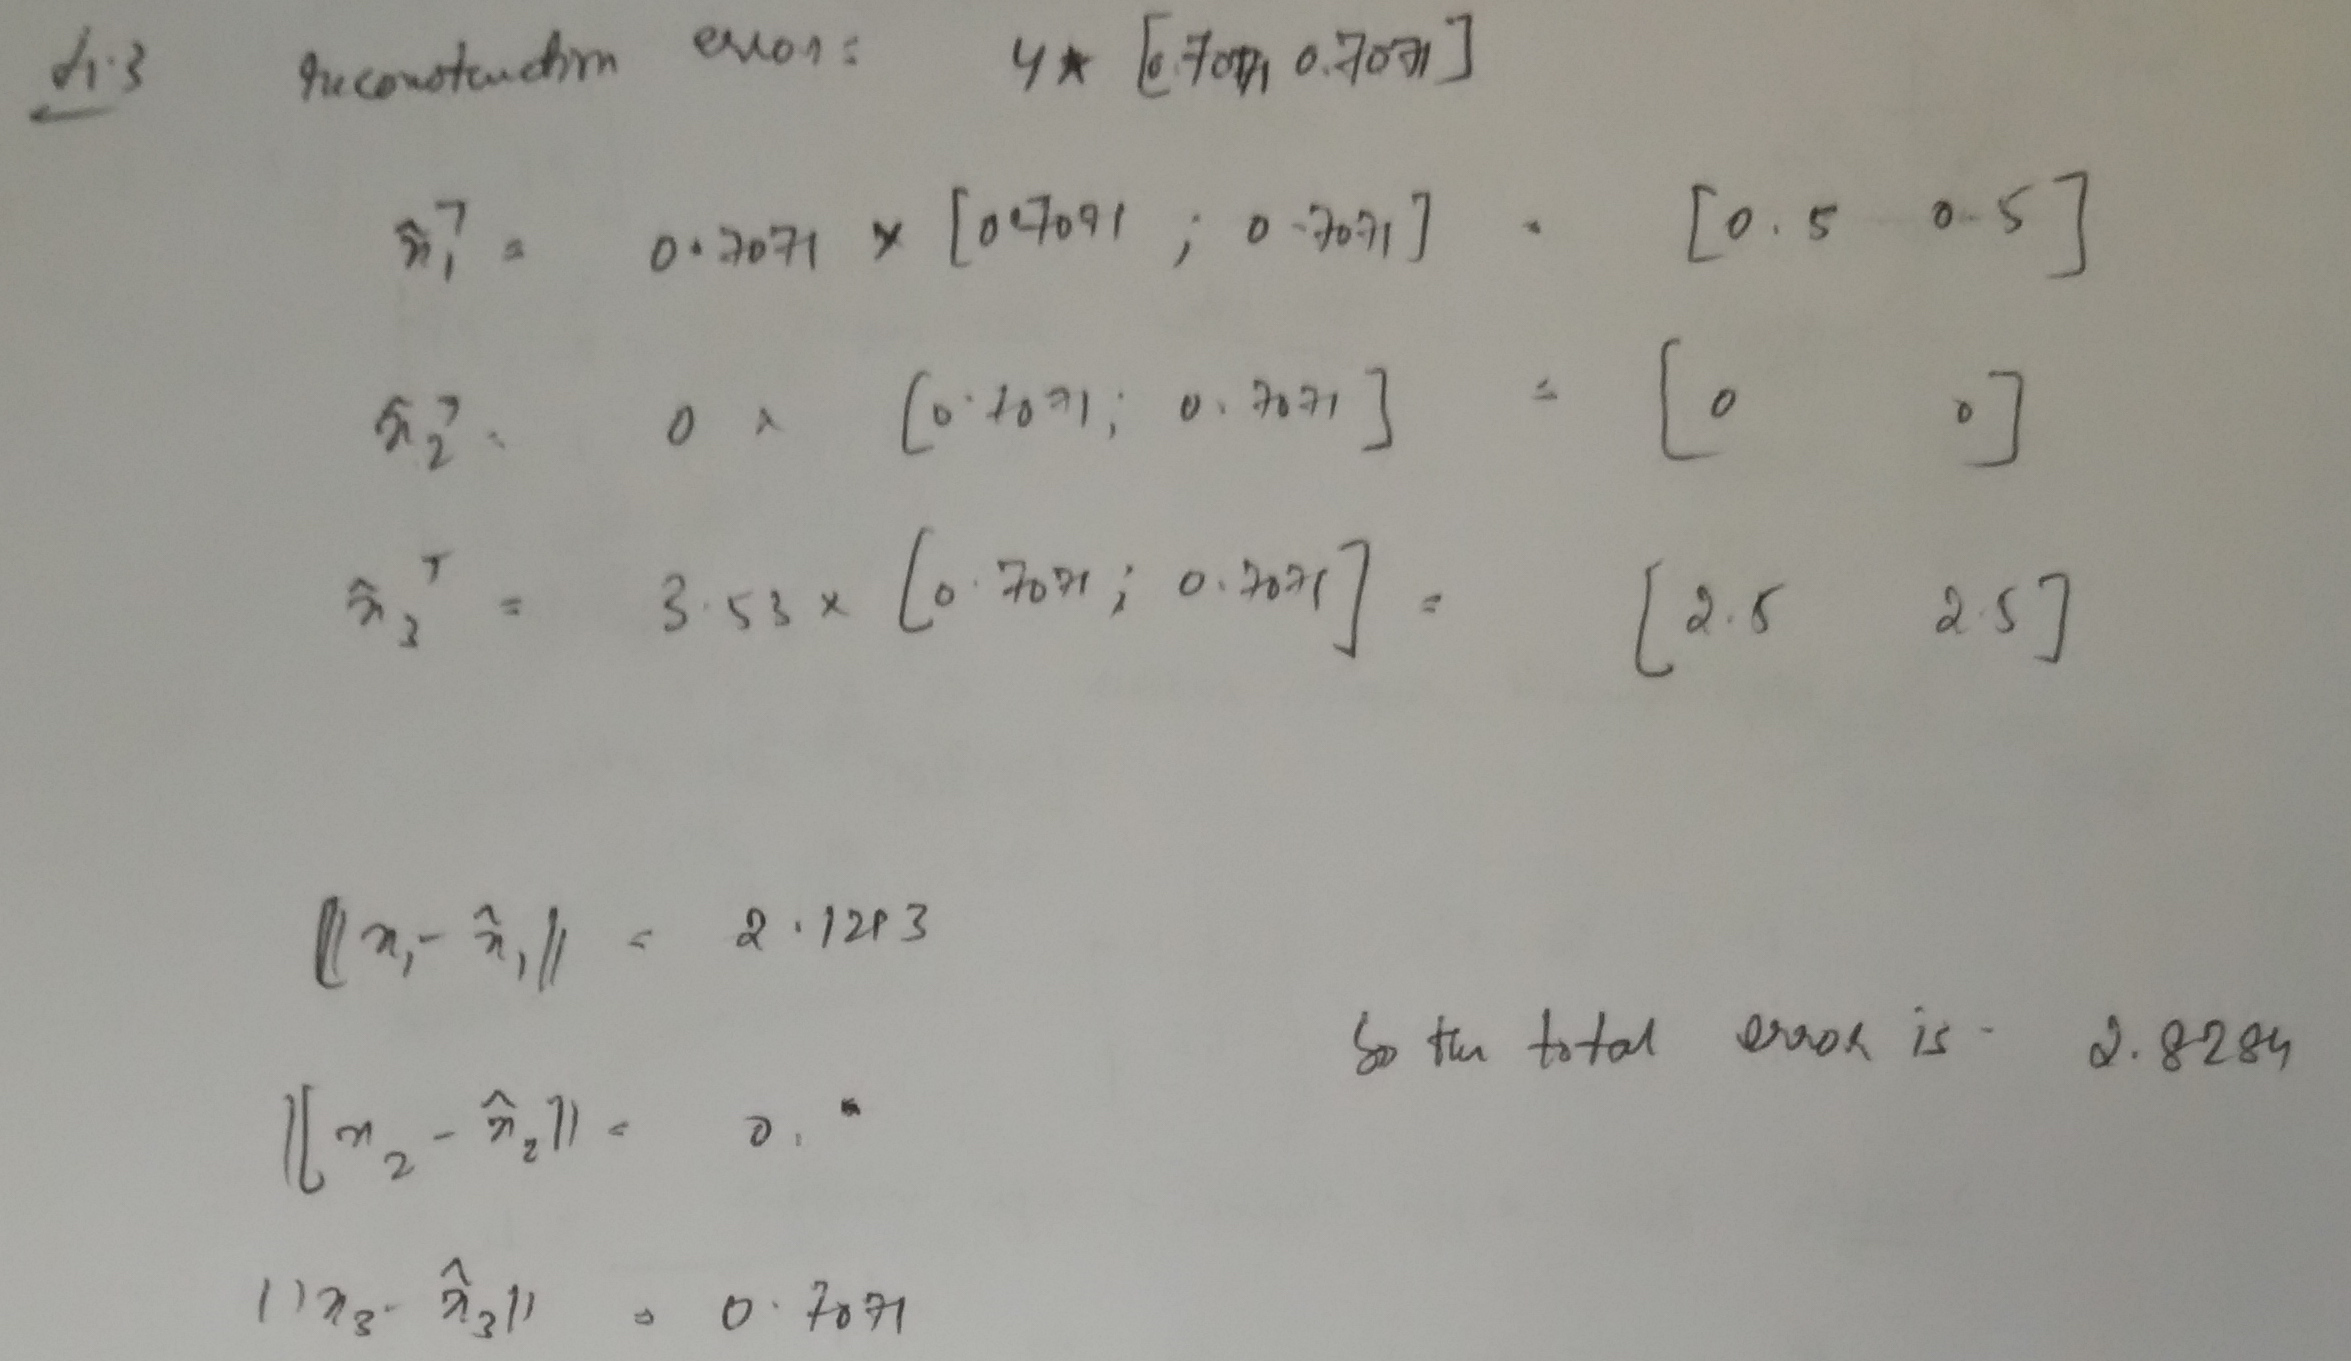
\includegraphics[width=\linewidth]{4_3.jpg}
	\caption{Q 4.3}
	\label{fig:Q 4.3}
\end{figure}
The error in fig \ref{fig:Q 4.3} is calculated with euclidean distance btw the two points. The matrix is reconstructed into the original 2D subspace with the principal component used to reduce the subspace. The new points are Xbar and the original points are X the distance between the two gives the reconstruction error for the point.

\end{document}